% ============================================================
%  Semana 6 · Clase 11: Principios de visualización y comunicación de datos
%  Curso: Análisis y Visualización de Datos para la Toma de Decisiones
%
%  Formato de la sesión (3 h):
%    Hora 1. Qué hace efectiva una visualización; selección del gráfico
%             según la pregunta: comparación, composición, distribución,
%             relación
%    Hora 2. Escalas, etiquetas, color y reducción de ruido visual
%    Hora 3. Errores comunes y gráficos engañosos; introducción al taller
%             en Colab (notebooks/lab-visualizacion.ipynb)
%
%  Compilar (dos veces) directamente desde esta carpeta:
%    xelatex semana06-clase11.tex
%    xelatex semana06-clase11.tex
% ============================================================
\documentclass[aspectratio=169,11pt]{beamer}

\usepackage{../../../plantilla/beamerthemeesumer}
\usetheme{esumer}

\usepackage[spanish]{babel}
\usepackage{booktabs}
\usepackage{graphicx}

% ---------------- DATOS DE LA CLASE ----------------
\title{Principios de visualización y comunicación de datos}
\subtitle{De la tabla resumen al gráfico que convence}
\author{Docente: Cristian A. Jimenez C., MSc}
\date{Oct 13 al 18}

\setmodulo{Módulo 2: Construir (Limpieza y Gestión de Datos)}
\setsemana{6}
\setclase{11}
\setfechaclase{Oct 13 al 18}
\setmodalidad{Virtual}
% -----------------------------------------------------

\graphicspath{{figuras/}}

\begin{document}

{
\setbeamertemplate{footline}{}
\begin{frame}[plain]
  \titlepage
\end{frame}
}

\begin{frame}{Agenda de hoy (3 horas)}
  \begin{columns}[T,onlytextwidth]
    \column{0.32\textwidth}
    \begin{block}{Hora 1}
      \small Qué hace efectiva una visualización y cómo elegir el gráfico
      según la pregunta
    \end{block}
    \column{0.32\textwidth}
    \begin{block}{Hora 2}
      \small Escalas, etiquetas, color y reducción de ruido visual
    \end{block}
    \column{0.32\textwidth}
    \begin{block}{Hora 3}
      \small Errores comunes y gráficos engañosos; taller en Google Colab
    \end{block}
  \end{columns}
  \vspace{0.4cm}
  \small Desde la Clase 9 sabes construir un cuadro de indicadores con
  \texttt{groupby}. Hoy aprendes a mostrarlo: las mismas cifras, bien o mal
  presentadas, cambian lo que tu audiencia entiende y decide.
\end{frame}

% ============================================================
\section{Hora 1: Elegir el gráfico}
% ============================================================
\begin{frame}{¿Qué hace efectiva una visualización?}
  \small
  Un gráfico es efectivo cuando tu audiencia entiende el mensaje
  \textbf{más rápido mirándolo que leyendo la tabla de números}. No es una
  decoración del resultado: es parte del análisis.
  \vspace{0.2cm}
  \begin{block}{Tres preguntas antes de abrir cualquier librería de gráficos}
    \small
    \begin{enumerate}
      \item ¿Qué \textbf{pregunta de negocio} estoy respondiendo?
      \item ¿Qué tipo de comparación necesita esa pregunta? (Sección
        siguiente)
      \item ¿Qué es lo \textbf{mínimo} que tengo que mostrar para que se
        entienda, sin nada de más?
    \end{enumerate}
  \end{block}
  \small Si no puedes nombrar la pregunta que responde tu gráfico, todavía
  no estás listo para hacerlo.
\end{frame}

\begin{frame}{Las cuatro preguntas que determinan el gráfico}
  \small
  Casi cualquier gráfico de negocio responde una de estas cuatro preguntas.
  Identificarla primero evita el error más común: elegir el gráfico que se
  ve bonito en vez del que se entiende rápido.
  \begin{center}
    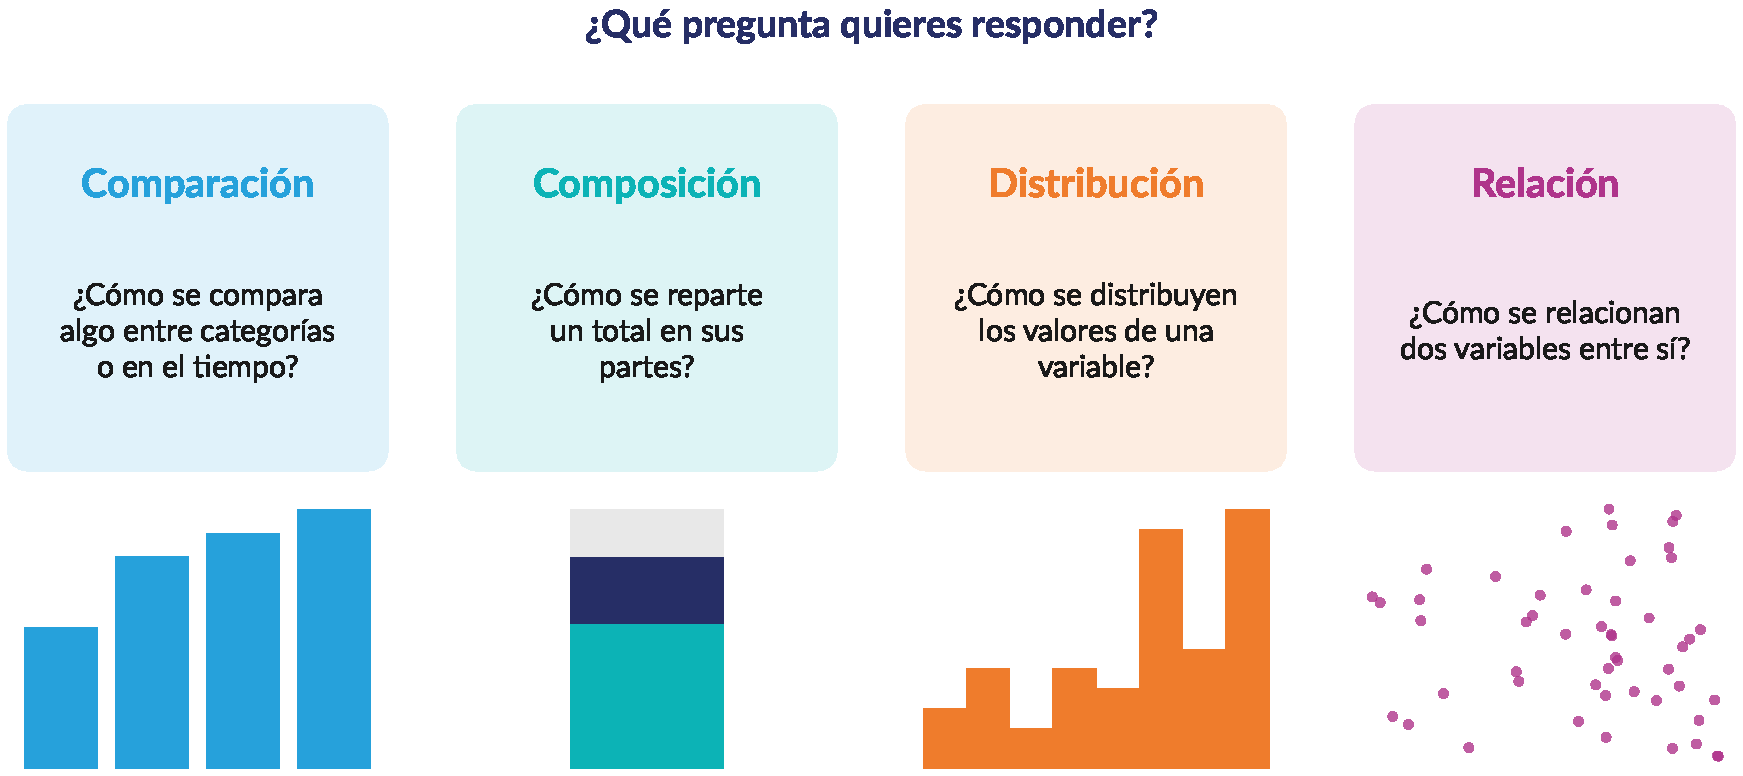
\includegraphics[width=0.74\textwidth,keepaspectratio]{figura_cuatro_preguntas.pdf}
  \end{center}
\end{frame}

\begin{frame}{Comparación}
  \small
  \textbf{Pregunta:} ¿cómo se compara algo entre categorías, o a lo largo
  del tiempo?
  \begin{columns}[T,onlytextwidth]
    \column{0.5\textwidth}
    \begin{exampleblock}{Pocas categorías, un momento}
      \small Barras verticales u horizontales. Ejemplo: socios por ciudad
      (Clase 9).
    \end{exampleblock}
    \column{0.5\textwidth}
    \begin{exampleblock}{Evolución en el tiempo}
      \small Línea. Ejemplo: inscripciones por mes (Clase 9, \texttt{dt.to\_period}).
    \end{exampleblock}
  \end{columns}
  \vspace{0.2cm}
  \small Regla práctica: con más de 10 a 12 categorías, una tabla ordenada
  suele comunicar mejor que un gráfico de barras saturado.
\end{frame}

\begin{frame}{Comparación: ejemplos con nuestros datos}
  \small
  \begin{center}
    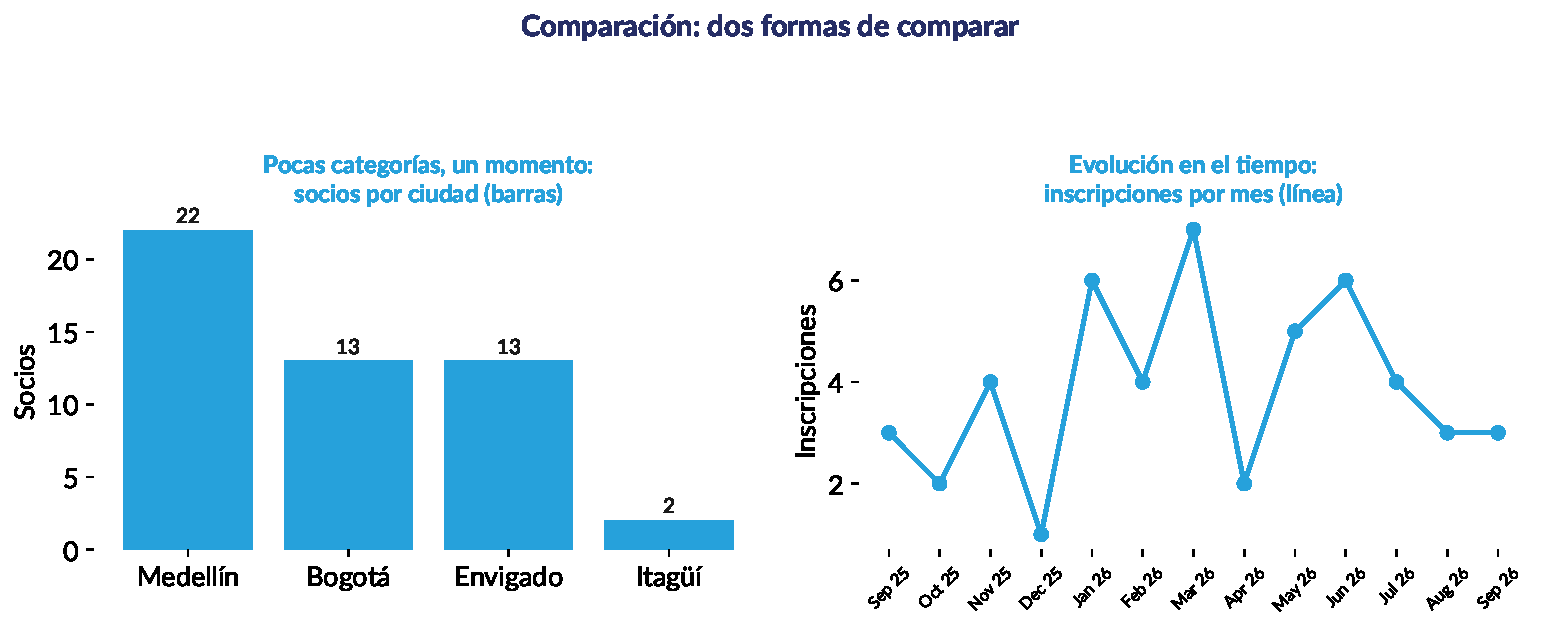
\includegraphics[width=0.92\textwidth,height=0.68\textheight,keepaspectratio]{figura_ejemplos_comparacion.pdf}
  \end{center}
\end{frame}

\begin{frame}{Composición}
  \small
  \textbf{Pregunta:} ¿cómo se reparte un total en sus partes?
  \begin{columns}[T,onlytextwidth]
    \column{0.5\textwidth}
    \begin{exampleblock}{Una sola composición}
      \small Barras apiladas, o un gráfico de pastel \textbf{solo} si hay
      pocas categorías (3 a 5) y la diferencia entre ellas es clara.
    \end{exampleblock}
    \column{0.5\textwidth}
    \begin{exampleblock}{Composición que cambia}
      \small Barras apiladas al 100\,\% por periodo, o varias barras
      apiladas una al lado de otra.
    \end{exampleblock}
  \end{columns}
  \vspace{0.2cm}
  \small Ejemplo del curso: participación de cada plan dentro de cada
  ciudad (Clase 9, \texttt{.transform("sum")}).
\end{frame}

\begin{frame}{Composición: ejemplos con nuestros datos}
  \small
  \begin{center}
    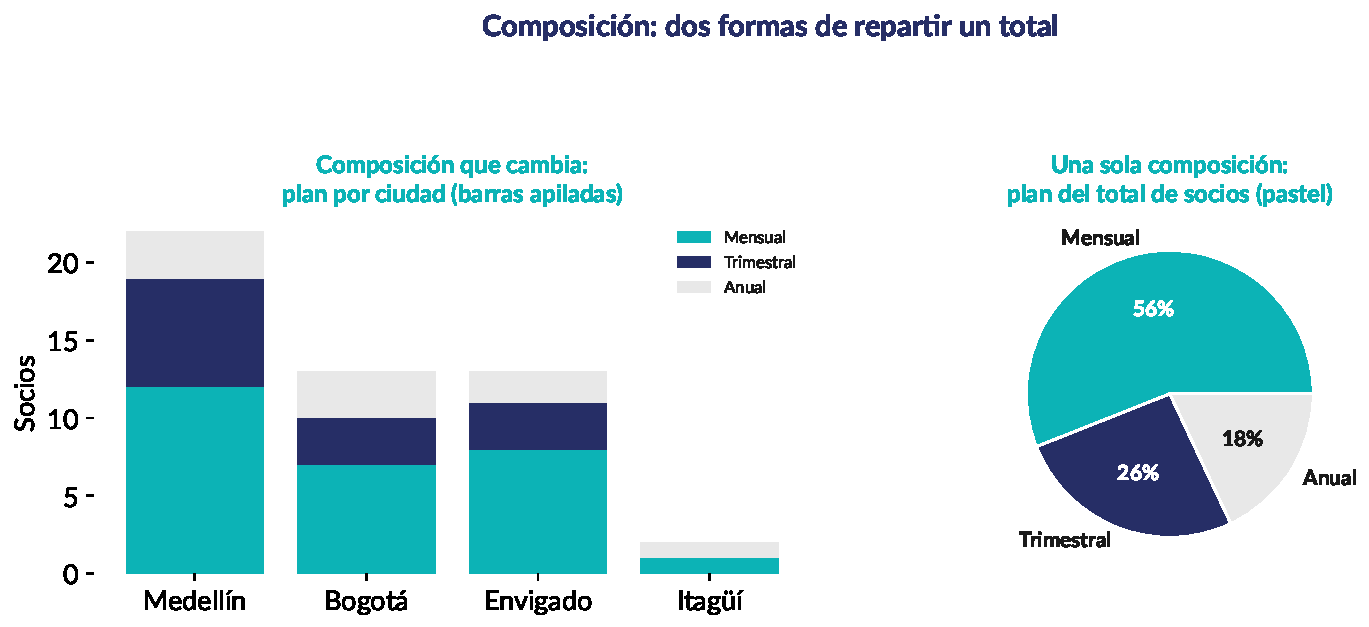
\includegraphics[width=0.92\textwidth,height=0.68\textheight,keepaspectratio]{figura_ejemplos_composicion.pdf}
  \end{center}
\end{frame}

\begin{frame}{Distribución}
  \small
  \textbf{Pregunta:} ¿cómo se distribuyen los valores de una variable?
  ¿Dónde se concentran, qué tan dispersos están, hay valores atípicos?
  \begin{columns}[T,onlytextwidth]
    \column{0.5\textwidth}
    \begin{exampleblock}{Una variable}
      \small Histograma (Clase 2): agrupa los valores en rangos y cuenta
      cuántas observaciones caen en cada uno.
    \end{exampleblock}
    \column{0.5\textwidth}
    \begin{exampleblock}{Comparar distribuciones}
      \small Boxplot (Clase 2): resume mediana, cuartiles y valores
      atípicos; útil para comparar varios grupos a la vez.
    \end{exampleblock}
  \end{columns}
  \vspace{0.2cm}
  \small Ejemplo del curso: la distribución de edades de los socios, o cómo
  se compara esa distribución entre planes.
\end{frame}

\begin{frame}{Distribución: ejemplos con nuestros datos}
  \small
  \begin{center}
    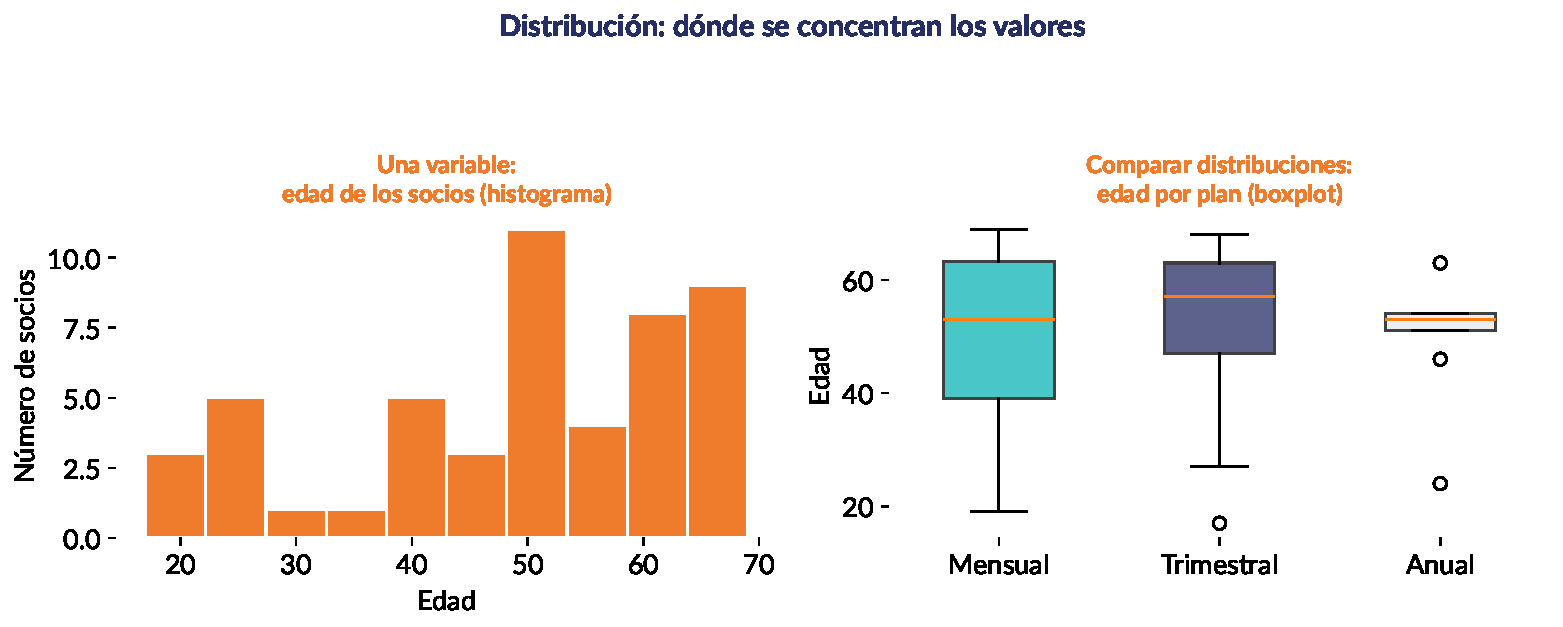
\includegraphics[width=0.92\textwidth,height=0.68\textheight,keepaspectratio]{figura_ejemplos_distribucion.pdf}
  \end{center}
\end{frame}

\begin{frame}{Relación}
  \small
  \textbf{Pregunta:} ¿cómo se relacionan dos variables entre sí? ¿Cuando
  una sube, la otra sube, baja, o no cambia?
  \begin{exampleblock}{Dos variables numéricas}
    \small Diagrama de dispersión (\textit{scatter}): cada punto es una
    observación, un eje por variable. La correlación de Pearson (Clase 2)
    la resume en un número; el gráfico te deja ver si esa relación es
    realmente lineal.
  \end{exampleblock}
  \small Recuerda la advertencia de la Clase 2: un valor de $r$ cercano a 0
  no significa ``no hay relación''; puede haber una relación fuerte que
  simplemente no es una línea recta. El gráfico de dispersión es la forma
  de comprobarlo.
\end{frame}

\begin{frame}{Relación: ejemplos con nuestros datos}
  \small
  \begin{center}
    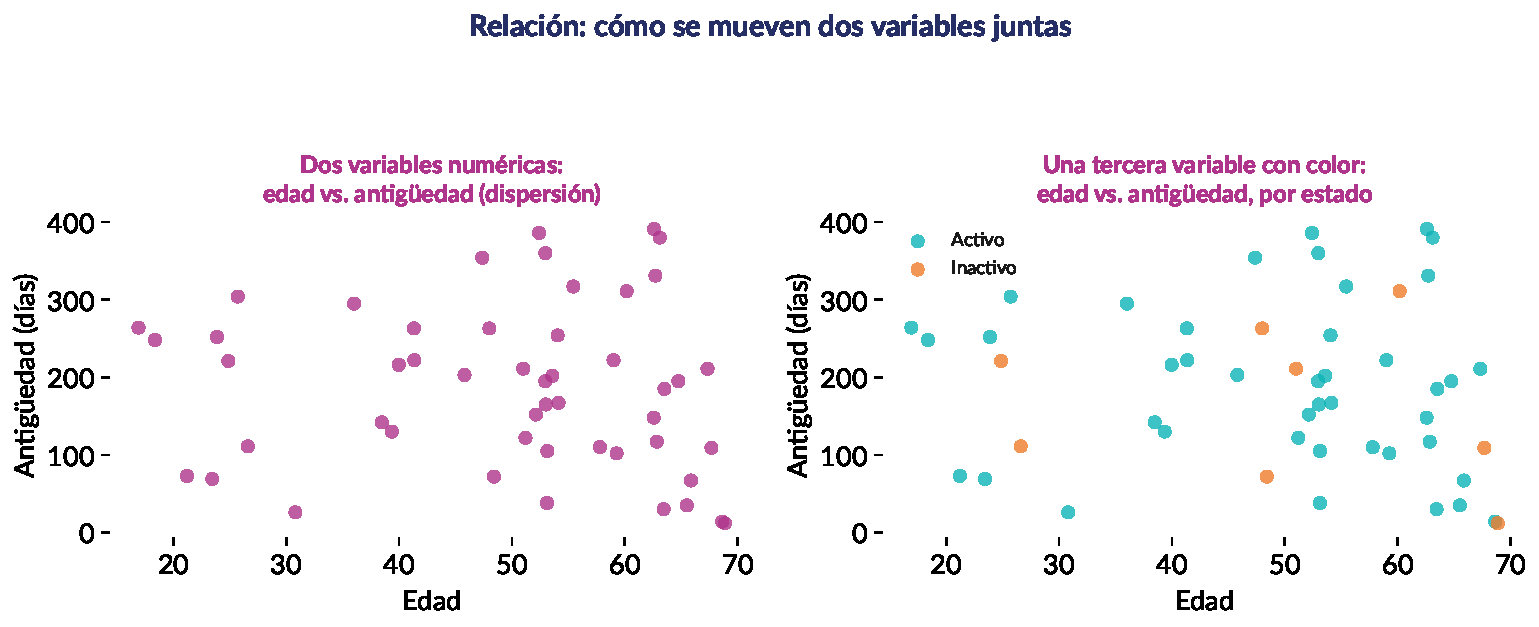
\includegraphics[width=0.92\textwidth,height=0.68\textheight,keepaspectratio]{figura_ejemplos_relacion.pdf}
  \end{center}
\end{frame}

% ============================================================
\section{Hora 2: Escalas, etiquetas, color y ruido}
% ============================================================
\begin{frame}{Escalas: el eje que decide lo que ves}
  \small
  El mismo dato, con un eje distinto, cuenta una historia distinta. Para
  gráficos de barras, el eje que mide la magnitud \textbf{debe empezar en
  cero}: el ojo compara el \textit{tamaño} de las barras, y truncar el eje
  rompe esa comparación.
  \begin{center}
    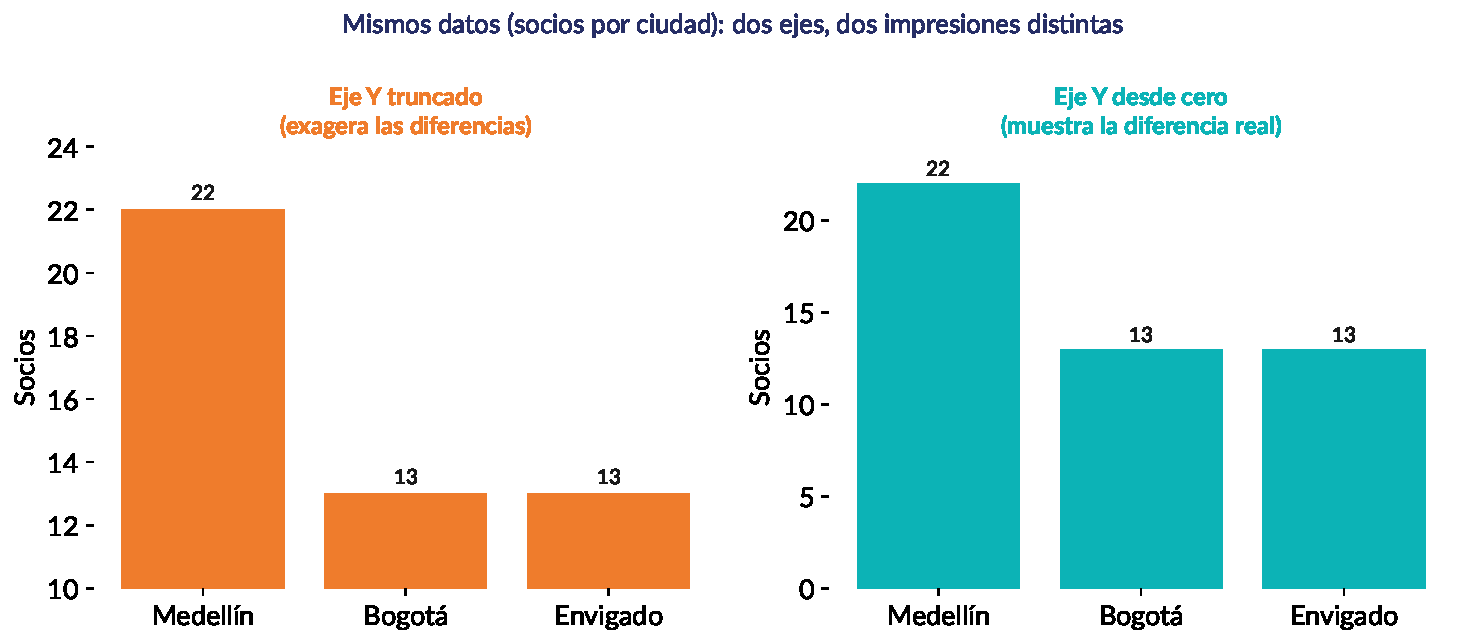
\includegraphics[width=0.92\textwidth]{figura_escala_eje.pdf}
  \end{center}
\end{frame}

\begin{frame}{¿Nunca se trunca un eje, entonces?}
  \small
  La regla ``empieza en cero'' es estricta para \textbf{barras} (donde el
  área y la altura son la comparación). Para \textbf{líneas} que muestran
  una tendencia en el tiempo, truncar el eje es aceptable y a veces
  necesario para ver el movimiento, siempre que:
  \begin{itemize}
    \small
    \item lo digas explícitamente (una nota al pie, o el rango del eje
      visible),
    \item no sea tu única forma de ``inventar'' una tendencia que no
      existe.
  \end{itemize}
  \begin{alertblock}{Pregunta de control}
    \small Si alguien solo mira la forma del gráfico, sin leer los números
    de los ejes, ¿se llevaría una impresión correcta?
  \end{alertblock}
\end{frame}

\begin{frame}{Una tendencia, truncada y sin truncar}
  \small
  Lo mismo pasa con una línea: quitarle el aire al eje hace que cualquier
  vaivén se vea como un cambio brusco. Son los mismos datos de
  inscripciones por mes que ya viste; aquí el único cambio es el rango del
  eje Y.
  \begin{center}
    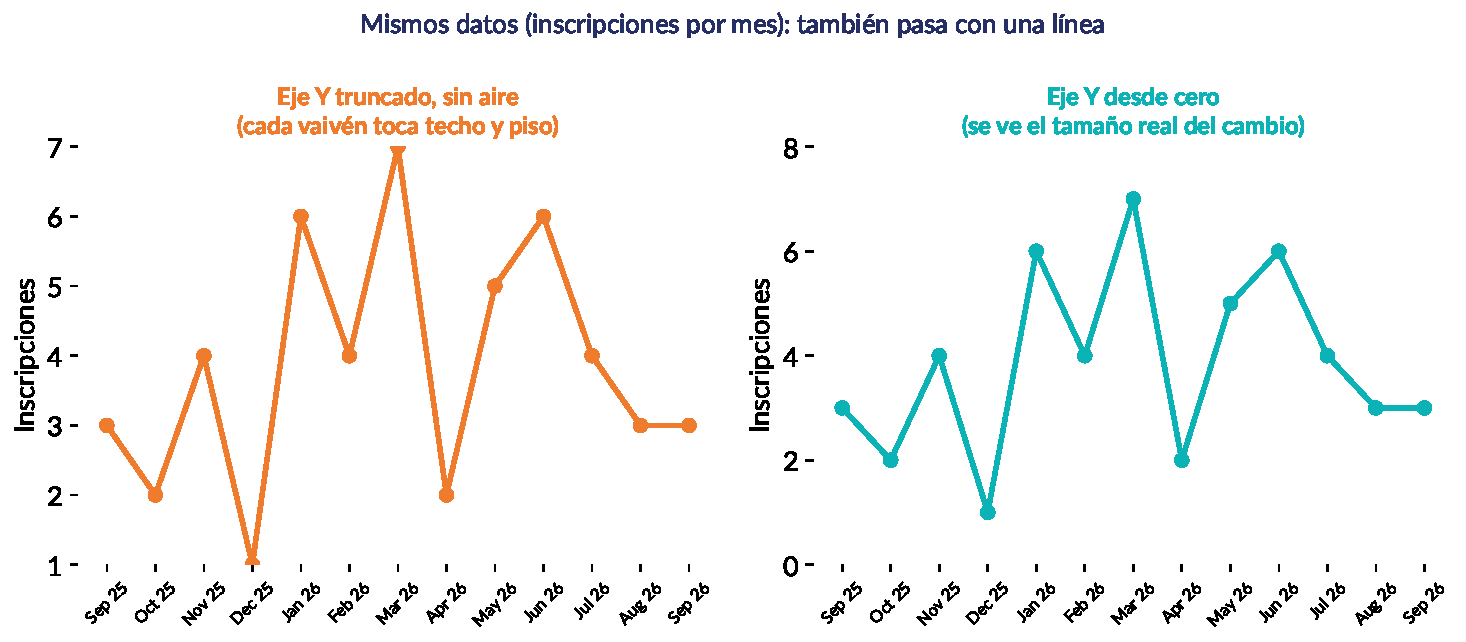
\includegraphics[width=0.92\textwidth,height=0.68\textheight,keepaspectratio]{figura_escala_linea.pdf}
  \end{center}
\end{frame}

\begin{frame}{Etiquetas: lo mínimo para que se entienda solo}
  \small
  Un gráfico bueno se entiende sin que tú estés al lado explicándolo.
  \begin{itemize}
    \small
    \item \textbf{Título}: la conclusión, no la descripción. Mejor
      ``Medellín concentra el 44\,\% de los socios'' que ``Socios por
      ciudad''.
    \item \textbf{Ejes}: nombre y unidad (\texttt{Socios}, no un número
      suelto).
    \item \textbf{Fuente y fecha}: de dónde salen los datos y de cuándo son.
    \item \textbf{Etiquetas directas sobre la barra o el punto}, en vez de
      una leyenda aparte, cuando hay pocas categorías: le ahorras a la
      audiencia ir y venir entre el gráfico y la leyenda.
  \end{itemize}
\end{frame}

\begin{frame}{Color: con propósito, no por decoración}
  \small
  \begin{columns}[T,onlytextwidth]
    \column{0.33\textwidth}
    \begin{exampleblock}{Categórico}
      \small Colores distintos sin orden entre ellos. Ejemplo: ciudad,
      plan. Máximo 5 a 6 colores: más que eso, nadie los distingue.
    \end{exampleblock}
    \column{0.33\textwidth}
    \begin{exampleblock}{Secuencial}
      \small Un solo color, de claro a oscuro. Para una variable que va de
      menos a más. Ejemplo: densidad, intensidad.
    \end{exampleblock}
    \column{0.33\textwidth}
    \begin{exampleblock}{Divergente}
      \small Dos colores que se alejan de un punto central. Para valores
      por encima o por debajo de un promedio, o positivos y negativos.
    \end{exampleblock}
  \end{columns}
  \vspace{0.2cm}
  \small Usa el color para \textbf{resaltar lo que importa}: una sola
  categoría en color y el resto en gris comunica más que diez colores
  compitiendo por la atención. Y revisa que tu paleta se distinga también
  para quienes tienen daltonismo (evita depender solo de rojo y verde).
\end{frame}

\begin{frame}{Las tres paletas, con un ejemplo real}
  \small
  Mismo dato (socios por ciudad), tres preguntas distintas según cómo uses
  el color: ¿qué ciudad es cada una, qué tanto tiene, o está por encima o
  por debajo del promedio?
  \begin{center}
    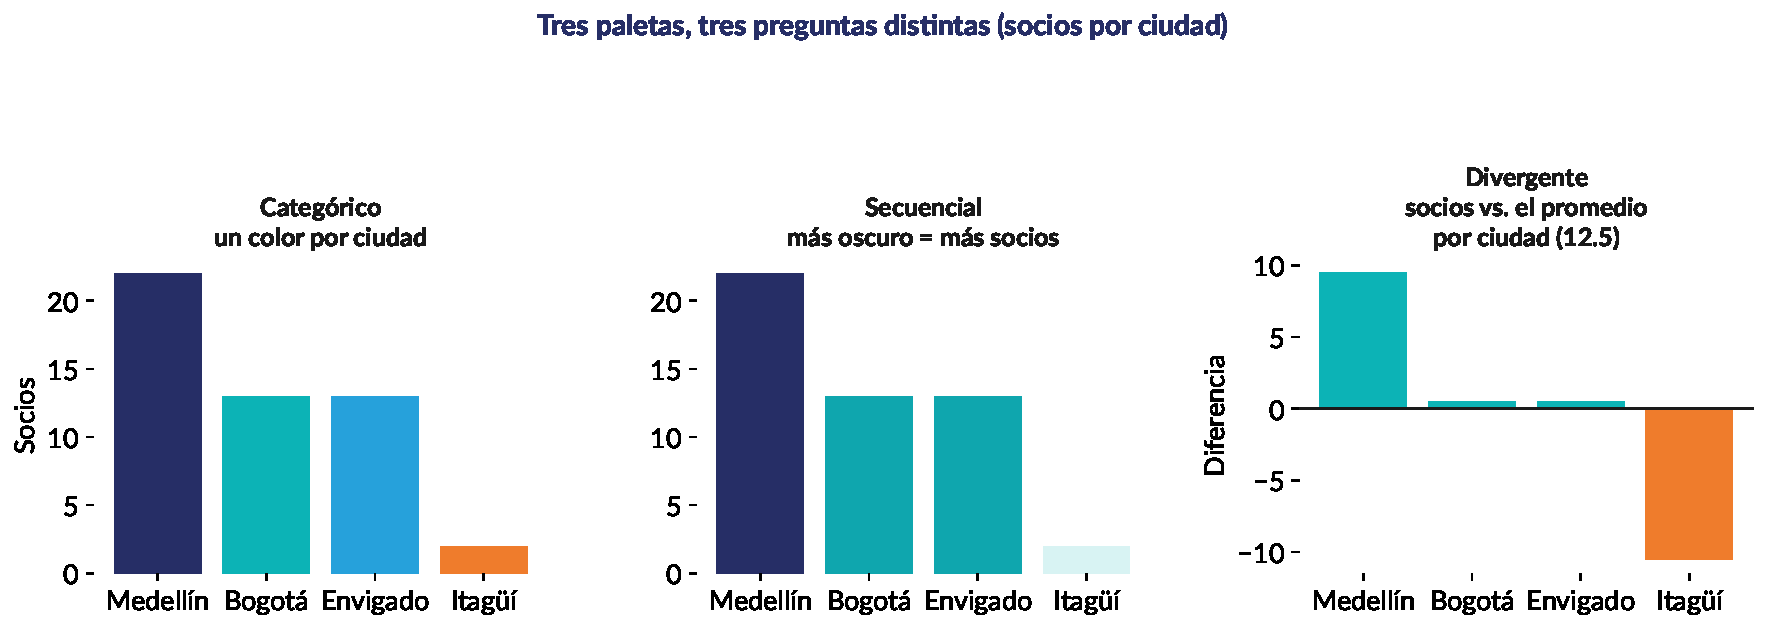
\includegraphics[width=0.95\textwidth,height=0.68\textheight,keepaspectratio]{figura_tipos_color.pdf}
  \end{center}
\end{frame}

\begin{frame}{Reducir el ruido visual}
  \small
  Edward Tufte lo resume con la idea de \textit{data-ink ratio}: la
  proporción del gráfico dedicada a mostrar datos, frente a todo lo demás
  (rejillas pesadas, bordes, sombras, efectos 3D). Cada elemento que no
  ayuda a leer el dato \textbf{compite} por la atención con el dato mismo.
  \begin{center}
    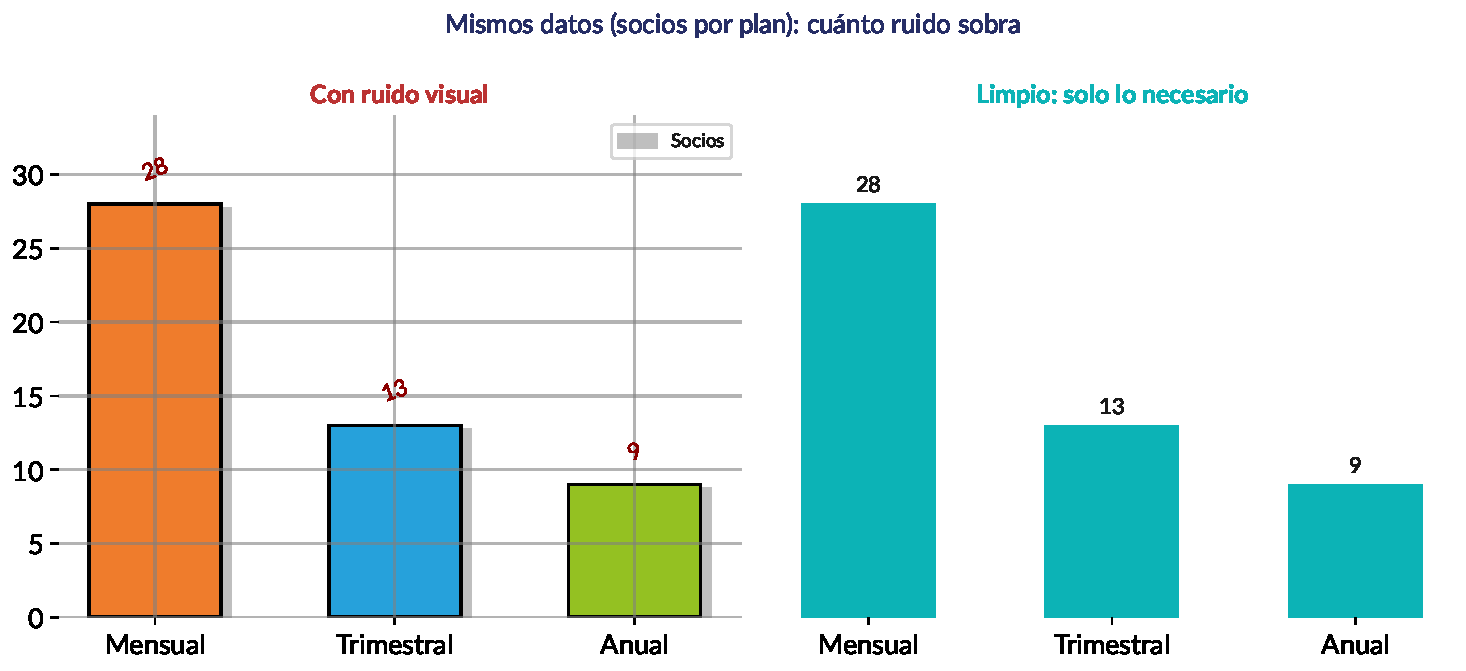
\includegraphics[width=0.92\textwidth]{figura_ruido_visual.pdf}
  \end{center}
\end{frame}

\begin{frame}{Checklist para quitar ruido}
  \small
  \begin{itemize}
    \small
    \item ¿Necesito rejilla de fondo, o las etiquetas de valor ya bastan?
    \item ¿Necesito leyenda, o puedo poner la etiqueta directamente sobre
      la barra o la línea?
    \item ¿Los bordes y las sombras de las barras agregan información?
    \item ¿Estoy usando 3D en un gráfico que es, en realidad, de dos
      dimensiones? (El 3D distorsiona el tamaño relativo: nunca lo uses
      para comparar magnitudes.)
    \item ¿Cada color que usé significa algo, o solo está ahí porque la
      herramienta lo puso por defecto?
  \end{itemize}
\end{frame}

% ============================================================
\section{Hora 3: Errores comunes y gráficos engañosos}
% ============================================================
\begin{frame}{El pastel es el gráfico más mal usado}
  \small
  El ojo humano compara \textbf{largos} mucho mejor de lo que compara
  \textbf{ángulos} o \textbf{áreas}. Por eso un gráfico de pastel con
  rebanadas parecidas es casi imposible de leer con precisión, mientras que
  las mismas cifras en barras se comparan de un vistazo.
  \begin{center}
    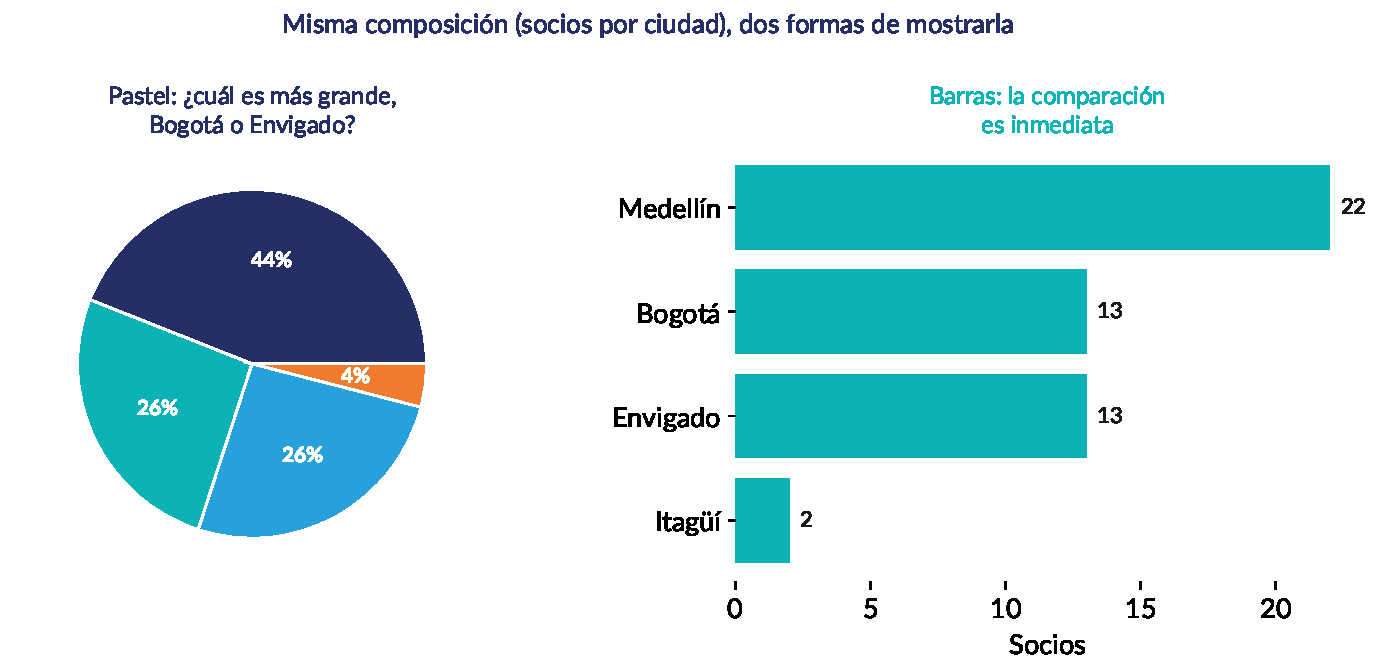
\includegraphics[width=0.92\textwidth]{figura_pie_vs_barras.pdf}
  \end{center}
\end{frame}

\begin{frame}{Doble eje Y: dos escalas, una sola impresión}
  \small
  Un gráfico de doble eje Y pone dos variables distintas en el mismo
  gráfico, cada una con su propio eje vertical, compartiendo el eje X.
  \begin{alertblock}{Por qué es tan fácil que engañe}
    \small Cada eje se ajusta, casi siempre en automático, al rango de
    \textbf{su propia} serie. El resultado es que las dos líneas terminan
    ocupando toda la altura del gráfico, sin importar si las variables
    tienen algo que ver entre sí. El ojo lee ``suben y bajan juntas''
    aunque la relación real sea nula.
  \end{alertblock}
  \small Regla práctica: si necesitas comparar dos variables en unidades
  distintas, casi siempre es más honesto mostrarlas en \textbf{paneles
  separados} (uno encima del otro, mismo eje X) que forzarlas en un solo
  gráfico con dos escalas libres.
\end{frame}

\begin{frame}{Ejemplo: inscripciones y edad promedio, mes a mes}
  \small
  Dos series reales de nuestros datos, prácticamente sin relación entre sí
  (correlación real $r = 0{,}03$). A la izquierda, el mismo gráfico de
  doble eje que verías por defecto en casi cualquier herramienta; a la
  derecha, las mismas series en paneles separados.
  \begin{center}
    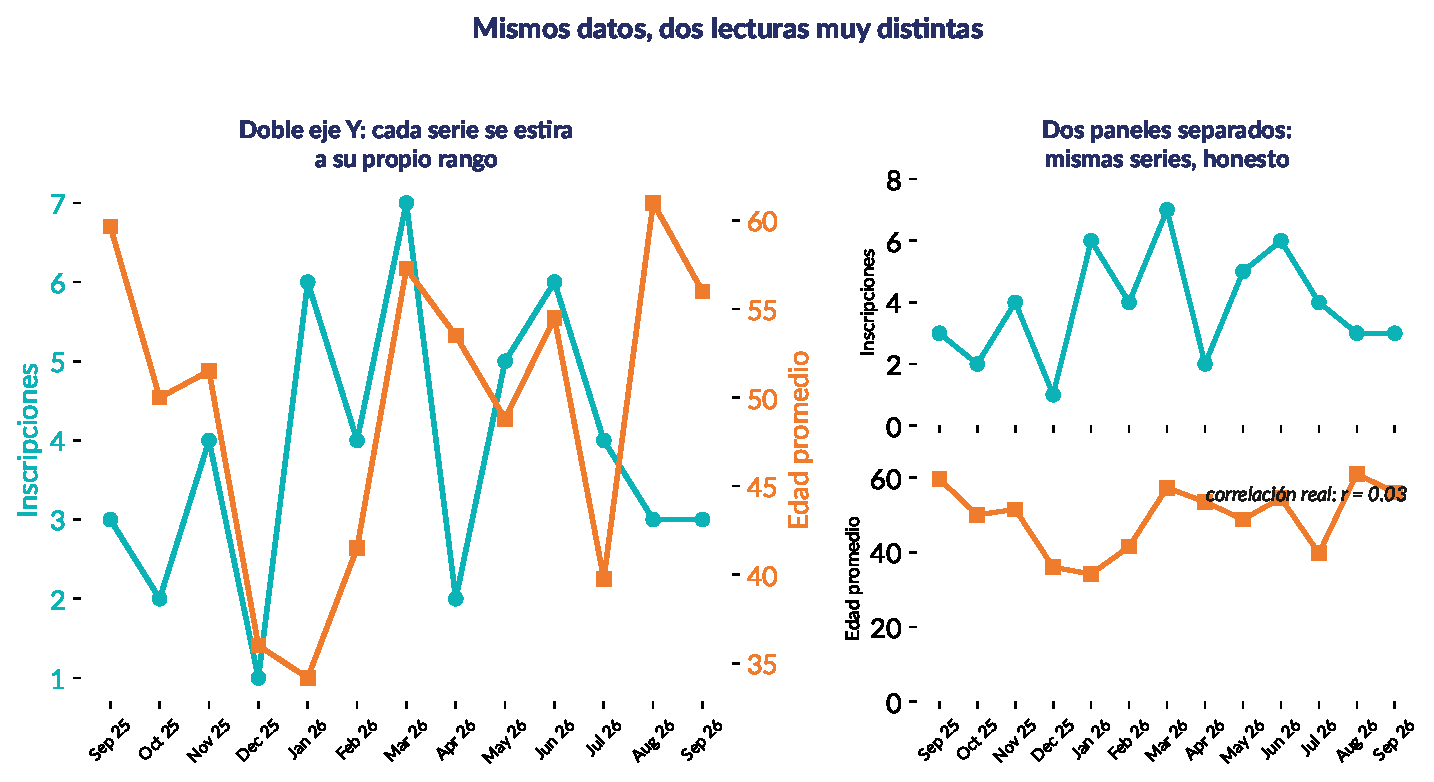
\includegraphics[width=0.95\textwidth,height=0.64\textheight,keepaspectratio]{figura_doble_eje.pdf}
  \end{center}
\end{frame}

\begin{frame}{Otros gráficos engañosos frecuentes}
  \small
  \begin{itemize}
    \small
    \item \textbf{Orden arbitrario}: categorías en el orden en que llegaron
      en el archivo, en vez de ordenadas por valor. Oculta el patrón que el
      gráfico debería mostrar.
    \item \textbf{Comparar cosas no comparables}: ya lo viste en la Clase
      8, al mezclar un precio mensual con uno anual sin llevarlos a la
      misma escala antes de graficar.
    \item \textbf{Promedios sin tamaño de muestra}: un promedio de 2
      observaciones (Itagüí, Clase 9) graficado junto a uno de 22 sin
      ninguna indicación de que no son igual de confiables.
  \end{itemize}
\end{frame}

\begin{frame}[allowframebreaks]{Otros gráficos que no vimos hoy}
  \small
  Barras, líneas, histograma, boxplot, dispersión y pastel cubren la
  mayoría de los casos, pero no todos.
  \begin{exampleblock}{Violín}
    \small Como el boxplot, pero muestra la forma completa de la
    distribución, no solo sus cuartiles.\\
    \href{https://seaborn.pydata.org/generated/seaborn.violinplot.html}{\color{esumerOrange}seaborn.violinplot →}
  \end{exampleblock}
  \begin{exampleblock}{Barras con barras de error}
    \small Un promedio junto con su incertidumbre (desviación estándar o
    intervalo de confianza).\\
    \href{https://matplotlib.org/stable/api/_as_gen/matplotlib.pyplot.errorbar.html}{\color{esumerOrange}matplotlib.pyplot.errorbar →}
  \end{exampleblock}
  \begin{exampleblock}{Mapa de calor}
    \small Dos categorías cruzadas, con color en vez de barras; útil
    cuando una tabla cruzada tiene demasiadas filas.\\
    \href{https://seaborn.pydata.org/generated/seaborn.heatmap.html}{\color{esumerOrange}seaborn.heatmap →}
  \end{exampleblock}
% \end{frame}

% \begin{frame}{Otros gráficos que no vimos hoy (2/2)}
%   \small
  \begin{exampleblock}{Área}
    \small Como una línea, pero con el espacio debajo relleno. Comunica
    bien una cantidad que se acumula en el tiempo.\\
    \href{https://matplotlib.org/stable/api/_as_gen/matplotlib.pyplot.fill_between.html}{\color{esumerOrange}matplotlib.pyplot.fill\_between →}
  \end{exampleblock}
  \begin{exampleblock}{Burbujas}
    \small Un gráfico de dispersión con una tercera variable codificada en
    el tamaño del punto, además de las dos de los ejes.\\
    \href{https://matplotlib.org/stable/api/_as_gen/matplotlib.pyplot.scatter.html}{\color{esumerOrange}matplotlib.pyplot.scatter →}
  \end{exampleblock}
  \begin{exampleblock}{Treemap}
    \small Composición con muchas categorías, donde el pastel ya no es
    legible: rectángulos de área proporcional.\\
    \href{https://plotly.com/python/treemaps/}{\color{esumerOrange}plotly: Treemap charts →}
  \end{exampleblock}
\end{frame}

\begin{frame}{Checklist final antes de publicar un gráfico}
  \small
  \begin{enumerate}
    \small
    \item ¿Qué pregunta responde? ¿Se nota con solo mirarlo?
    \item ¿Elegí el tipo de gráfico según esa pregunta (Hora 1), no por
      costumbre?
    \item ¿El eje de magnitud empieza en cero, o expliqué por qué no?
    \item ¿Tiene título, ejes con unidad, y fuente?
    \item ¿Cada color significa algo?
    \item ¿Quité todo lo que no ayuda a leer el dato?
  \end{enumerate}
  \vspace{0.2cm}
  \begin{alertblock}{Antes de compartirlo}
    \small Muéstraselo a alguien que no conozca los datos, durante 5
    segundos. Si no puede decirte el mensaje principal, el gráfico todavía
    no está listo.
  \end{alertblock}
\end{frame}

\begin{frame}{Actividad práctica}
  \begin{alertblock}{Taller de la sesión}
    \small En Google Colab vas a construir, paso a paso, los tipos de
    gráfico de esta clase con matplotlib y pandas sobre datos reales del
    curso. Al final del notebook hay un taller: rediseñar tres gráficos
    deficientes y justificar, con lo visto hoy, cada decisión de rediseño.
  \end{alertblock}
  \small El notebook incluye enlaces a la documentación oficial (en
  español e inglés) de cada tipo de gráfico, para que los uses como
  referencia en tus propios proyectos.
\end{frame}

\begin{frame}{Producto esperado}
  \begin{exampleblock}{Entregable}
    \small El notebook completo de la sesión: las celdas guiadas de cada
    tipo de gráfico, y el taller final con los tres gráficos rediseñados,
    cada uno con una justificación escrita de qué principio de esta clase
    aplicaste y por qué.
  \end{exampleblock}
\end{frame}

% ============================================================
\section{Cierre}
% ============================================================
\begin{frame}{Cierre y próxima sesión}
  \begin{itemize}
    \item Un gráfico efectivo responde una pregunta concreta, con el tipo
      de gráfico correcto para esa pregunta.
    \item Escalas honestas, etiquetas completas, color con propósito y sin
      ruido visual son lo que separa un gráfico que informa de uno que
      solo decora.
    \item Los gráficos engañosos casi nunca son mentiras explícitas: son
      decisiones de diseño (un eje, un orden, un tipo de gráfico) que
      cambian la impresión sin cambiar los datos.
    \item Próxima sesión, \textbf{Clase 12, MasterClass}: recapitulación
      presencial del Módulo 2 completo (Pandas, integración de fuentes y
      visualización) antes de entrar al Módulo 3 (Power BI).
  \end{itemize}
\end{frame}

\begin{frame}{Referencias para seguir explorando}
  \small
  Dos recursos gratuitos, en línea, para consultar tipos de gráfico y
  principios de visualización más allá de lo que vimos hoy.
  \begin{columns}[T,onlytextwidth]
    \column{0.5\textwidth}
    \centering
    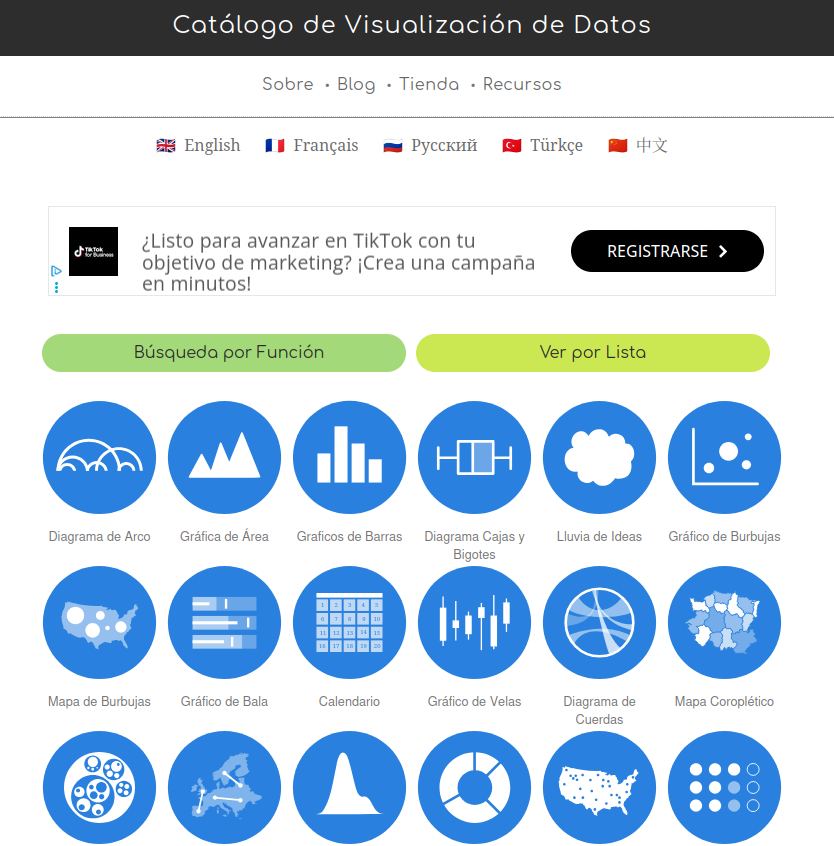
\includegraphics[width=0.8\textwidth,height=3.9cm,keepaspectratio]{captura_datavizcatalogue.png}\\[0.2cm]
    \begin{minipage}{0.92\textwidth}
      \small\textbf{Data Viz Catalogue} (en español): catálogo visual de
      tipos de gráfico, con qué es, cuándo usarlo y qué variaciones
      existen.\\
      \href{https://datavizcatalogue.com/ES/}{\color{esumerOrange}datavizcatalogue.com/ES →}
    \end{minipage}

    \column{0.5\textwidth}
    \centering
    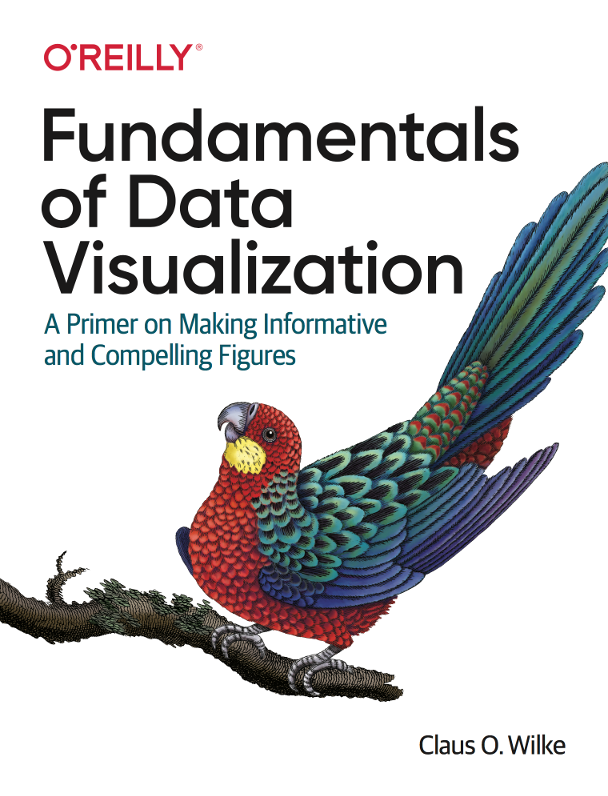
\includegraphics[height=3.9cm,keepaspectratio]{portada_fundamentals_dataviz.png}\\[0.2cm]
    \begin{minipage}{0.92\textwidth}
      \small\textbf{Fundamentals of Data Visualization}, Claus Wilke: libro
      completo y gratuito sobre los principios de hoy (selección del
      gráfico, color, escalas). En inglés.\\
      \href{https://clauswilke.com/dataviz/index.html}{\color{esumerOrange}clauswilke.com/dataviz →}
    \end{minipage}
  \end{columns}
\end{frame}

{
\setbeamertemplate{footline}{}
\begin{frame}[plain]
  \begin{tikzpicture}[remember picture,overlay]
    \fill[esumerNavy] (current page.south west) rectangle (current page.north east);
    \node at (current page.center) {\color{white}\Huge\bfseries ¡Gracias!};
  \end{tikzpicture}
\end{frame}
}

\end{document}
